\chapter{Experiments}
\label{Chapter5}
\settocdepth{subsection}
The majority of our experiments focuses on weighting the watershed locations. That corresponds to the \textbf{Structured voting (SV)} stage of the pipeline SE-SV-UCM, which we propose in \cref{Chapter4} for the task of going from edges to contours.

\textbf{Dataset:} For the evaluation of our segmentation results we work on the Berkeley Segmentation Data Set (BSDS500)~\cite{Arbelaez11}. Since its introduction in 2001, it has by now become a standard dataset for both the task of edge detection as well as that of image segmentation.

\textbf{Benchmark:} We report results on the benchmark~\cite{Galasso13Benchmark} introduced in~\cite{Galasso13} which can evaluate segmentation hierarchies against given ground-truth segmentations. It demonstrates the tradeoff between an oversegmentation and a more accurate object-centric segmentation.

\textbf{Watershed weighting strategy:} The Structured voting requires a choice of a watershed weighting strategy. The purpose of the weighting is associating a \textbf{score} with each of the watershed locations pixels. That score must faithfully reflect the strength of the underlying boundary. So we want to evaluate how good is the boundary evidence presented by the most likely segmentation determined by the structured forest. 

The first aspect of our voting strategy is making the structured forest patch and the watershed locations patch comparable. The watershed patch is an oversegmentation, and in this sense, contains much more information, not exclusively about the location of the boundary that we would like to evaluate. So we strive to simplify the watershed patch, keeping only important information about it - the shape of the boundary under consideration, or the constitution of the segmentation in the patch. Such a simplification in the context of our algorithm we call {\bf watershed patch transformation}. %``watershed patch transformation''. 

The second particular to a watershed weighting strategy is the choice of a scoring function. We view the task as a segmentation benchmark problem, where one of the patches is the ground truth segmentation, and the other - the segmentation under test. We analyse and apply a selection of boundary- and region- based metrics.

In the rest of the chapter we briefly describe the dataset and evaluation metrics used, in order to help understand the experiments. Afterwards, we give a detailed account of our most important experiments and the conclusions we draw based on them.

\section{Evaluation setup}
\subsection{Dataset}
\label{sec:ch5-BSDS500-dataset}
The Berkeley Segmentation Data Set (BSDS), introduced in~\cite{Martin01}, is a large dataset of natural images that have been manually segmented by multiple participants. It, therefore, provides the ground truth label for each pixel as being on- or off-boundary. Initially the dataset featured 300 images (BSDS300). It was later extended - in the new dataset BSDS500~\cite{Arbelaez11} the original 300 images are used for training (200) and validation (100), and 200 new human-annotated images are added for testing. Again, each image is segmented by different subjects. See \fref{fig:BSDS-annotations} for an example image and two of its annotations by different people.

\begin{figure}[ht!]
\begin{center}
  \begin{tabular}{ c c c }
  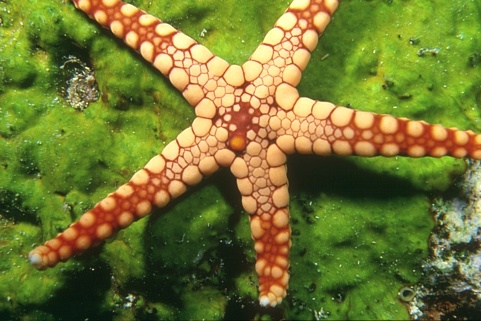
\includegraphics[width=0.3\textwidth]{images/examples/starfish/starfish.png} &
  
\includegraphics[width=0.3\textwidth,frame]{images/examples/starfish/starfish_bdry_coarse.png} &
  
\includegraphics[width=0.3\textwidth]{images/examples/starfish/starfish_segm_coarse.png} \\
  &
  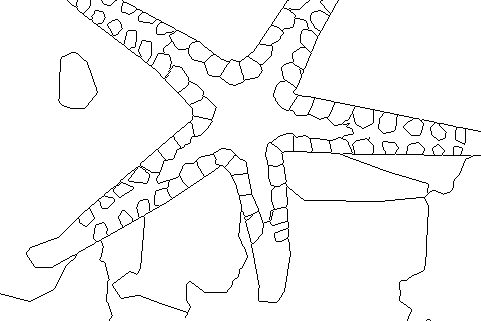
\includegraphics[width=0.3\textwidth,frame]{images/examples/starfish/starfish_bdry_detail.png} &
  
\includegraphics[width=0.3\textwidth]{images/examples/starfish/starfish_segm_detail.png} \\
  Input image & Boundaries & Segmentation \\
  \end{tabular}
\end{center}
\caption[BSDS500 dataset - 2 annotations]{Image from the validation subset of~\cite{BSDS500resources} and two of its annotations - subject~1 on the first row, subject~2 on the second row. {\bf Human-marked boundaries} are the central column, and their corresponding {\bf segmentation} reconstructions are given next to them.}
\label{fig:BSDS-annotations}
\end{figure}

\subsection{Metrics}
The benchmark that we use provides, among others, two precision-recall metrics - a boundary and a region oriented one.

\subsubsection{BPR}
The Boundary Precision-Recall (BPR)~\cite{Arbelaez11} is a boundary-based metric and emphasises the correct placement of image edges. Section~\ref*{sec:ch4-boundary-and-region-metrics-maths}~\ref{par:ch4-BPR-maths} % avoid having both links by using ref*
gives mathematical account on the metric and its properties. In case of segmentation, BPR is a good indicator of the {\bf localisation of the region boundaries}.

\textbf{Impact of %small 
local change in the boundary on the score:} A difference in the score of a single region boundary pixel should not greatly affect the edge detector output. Therefore, it correctly has only a small impact on the BPR metric. For the task of image segmentation however, a change in the strength of a single pixel could result in merging neighbouring regions. A ``weaker'' pixel among a strong intervening boundary could be thought as a leakage, which will cause the UCM algorithm (featured in \sref{sec:ch3-UCM}) % TODO give the algorithm in an appendix
to merge the two regions. In the hierarchical image segmentation framework, that means multiple levels of the segmentations hierarchy would change. So a rigorous image segmentation benchmark metric should not be oblivious to such changes.

\subsubsection{VPR}
To address the above issue, the other metric that we report is the Volume Precision-Recall (VPR) introduced by Galasso \etal~\cite{Galasso13} to evaluate the accuracy of video segmentation algorithms. For images (or video still frames) the metric is a region-based metric, operating % applied
into a precision-recall framework. It is measuring the size of the regions and the overlap between the ground truth segmentation regions and the segmentation regions produced by the algorithm under test. 
See Section~\ref*{sec:ch4-boundary-and-region-metrics-maths}~\ref{par:ch4-VPR-maths} for the formulae and discussion on the need for normalisation when evaluating segmentations.

% \section{Weighting strategies} % Exploration of the Space of Weighting Strategies}
% \section{Oracle} %  - Experiments with Ground Truth}
% \subsection{Oracle definition} % description}
% \subsection{Ranking of oracles}
% % \subsubsection{Confirms Correct Weighting Strategies}
% % \subsubsection{Failure Cases}

\subsubsection{Reported numbers}
\paragraph{For the precision-recall metrics BPR and VPR}\mbox{}\\\mbox{}\\
Both BPR and VPR are able to evaluate {\bf individual segmentations} (which on the plots are depicted as a single dot - the model error), as well as {\bf segmentation hierarchies}, represented using the UCM data structure (which on the plots constitute a curve). As stated in \sref{sec:ch4-boundary-and-region-metrics-maths}, for a single segmentation instance, the harmonic mean of the precision and recall, called the {\it F measure}, is reported. $F=\frac{2PR}{P+R}$.

In case of a probability of boundary, or a hierarchy of segmentations, which is in fact the case in the majority of our experiments, globally optimal scores %- best over the whole hierarchy, 
are reported. The scores are 3 in total: a best F-score (according to two criteria), as well as Average precision (\textbf{AP}). 

Optimal dataset score ({\bf ODS}) is the highest F score achieved while having a fixed scale for all images in the test set. 
Optimal image scale ({\bf OIS}) for BPR, or Optimal segmentation scale (\textbf{OSS}) for VPR is the average of the best F scores when allowing optimal scale {\it per image}. Hence, OIS\slash OSS is no lower than ODS. 
{\bf AP} is the precision averaged on the recall range $R\in[0,1]$, or, alternatively, the area under the precision-recall curve (AUC).

% TODO check if the following statement about ROC is indeed true
Note that in the case of edge detection benchmarked with BPR, P is not a function of R. Both values are {\bf functions of the segmentation threshold}. Thus it is possible to have different precision and same recall - on different threshold of detail, \ie different locations along the curve.
Not to be confused with %Compare with 
the receiver operating characteristic (ROC), used in statistics for comparing true-positive rate (TPR) against false-positive rate (FPR) of a binary classifier at various thresholds. In the ROC curve the TPR %sensitivity 
is a function of the FPR. %fall-out

\paragraph{Further region metrics}\mbox{}\\\mbox{}\\
Beside the aggregate measures for BPR and VPR, for the segmentation algorithms we also report the following region statistics. %(SC, PRI, VI)
\subparagraph{Segmentation covering of ground truth (SC):} This metric is an estimation of the best covering of the ground truth by the machine segments. We reviewed the metric in Section~\ref*{sec:ch4-boundary-and-region-metrics-maths}~\ref{par:ch4-SC-maths}.

\subparagraph{Probabilistic Rand index (PRI):} The PRI~\cite{UnnikrishnanPH07} is an extension of Rand index (RI)~\cite{rand1971objective}. It allows to assess the consistency of labelling of pixel pairs between the segmentation algorithm under test on one hand, and {\it multiple} ground truth segmentations on the other hand. Further, PRI partially addresses the issue of small dynamic range that RI displays. See Section~\ref*{sec:ch4-boundary-and-region-metrics-maths}~\ref{par:ch4-PRI-maths} for the formulae.

\subparagraph{Variation of information (VoI):} The Variation of information (VoI), introduced in~\cite{Meila05} measures the distance between two clusters of data - in our case, the human annotated and the machine-generated segmentation. The distance is measured \wrt %, in terms of 
their average conditional entropy and mutual information. This is the only metric that we report, which has preference for lower score, 0 being the theoretical best in case of equivalent segmentations.

\textbf{General preference:} For all metrics but VoI the general preference is ``higher is better''.

\paragraph{Example comparison of SE and gPb-OWT-UCM}\mbox{}\\\mbox{}\\
\tref{tab:SE_vs_gPb_OWT_UCM} has all the scores we just described, and \fref{fig:SE_vs_gPb_OWT_UCM} - the BPR and VPR plots for the two methods that we previously dissected - Structured edge~\cite{DollarICCV13edges} in \cref{Chapter2}, and gPb-OWT-UCM~\cite{Arbelaez11} in \cref{Chapter3}. 

Note that as SE is an edge detection algorithm, none of the region metrics or the VPR are applicable to its output. Since gPb-OWT-UCM is an image segmentation algorithm, the boundaries of the segments in a segmentation constitute closed contours, so boundary-based metrics, such as BPR, are applicable.

\begin{figure}[ht!]
\centering
 \subfigure[BPR]{%
  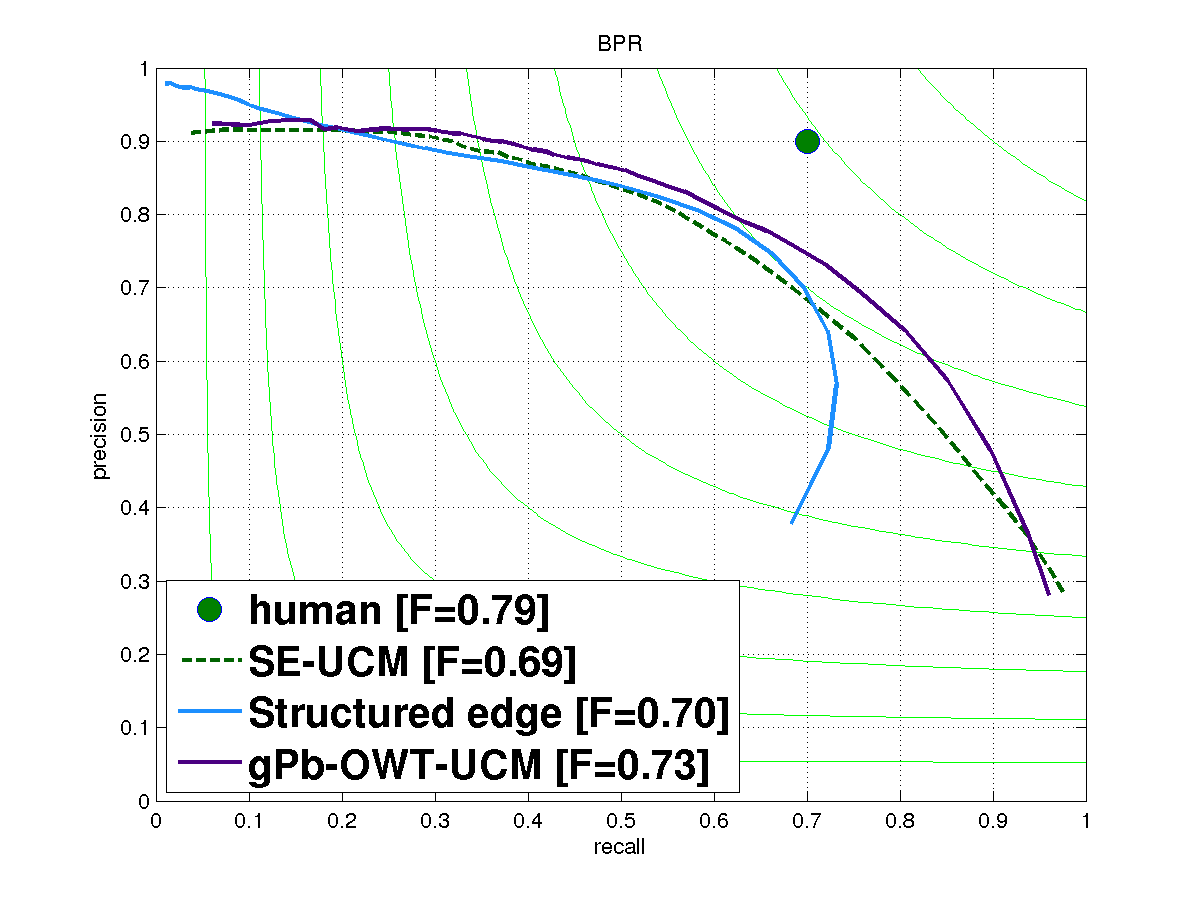
\includegraphics[trim=1.5cm 0cm 1.9cm 0cm, clip=true, width=0.48\textwidth]{images/plots/SE_vs_gPb_OWT_UCM_BPR.png}
 }
 \subfigure[VPR]{%
  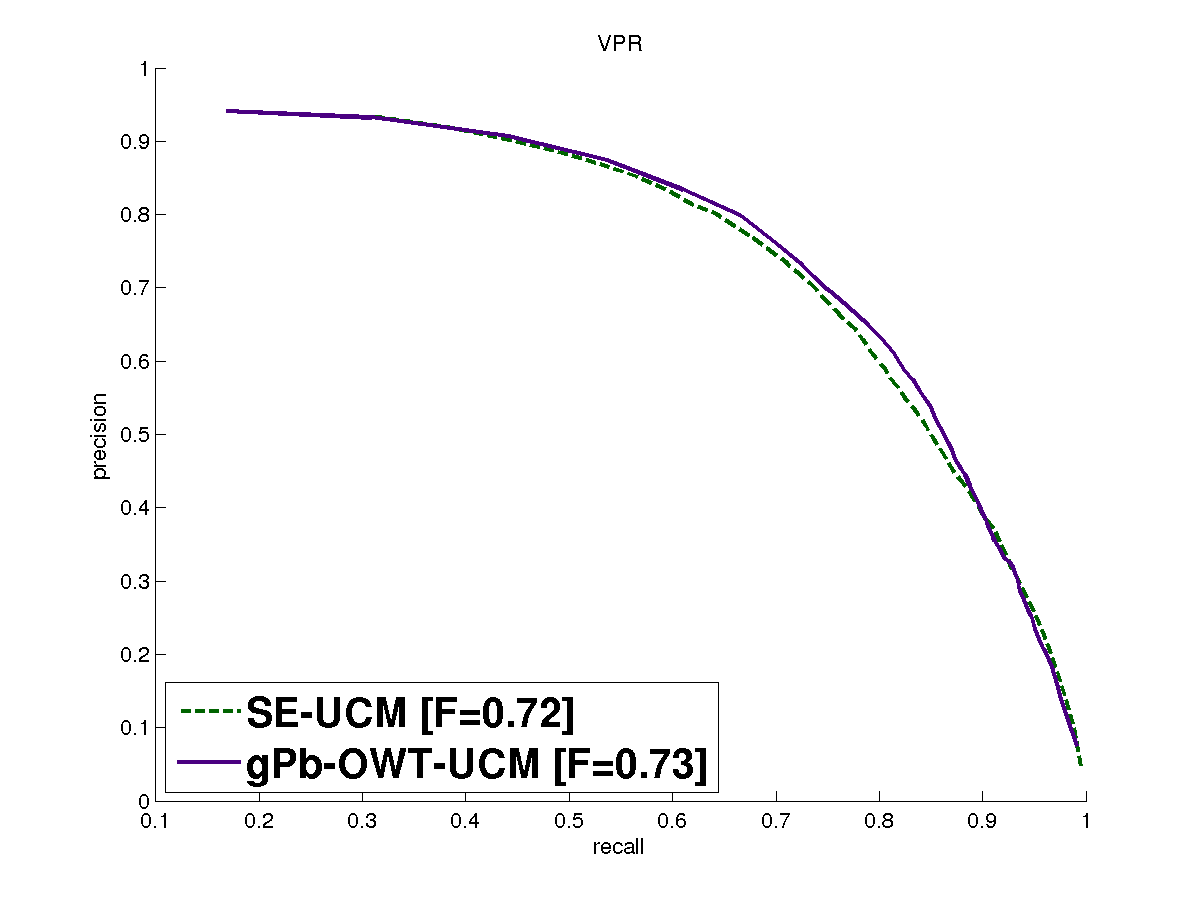
\includegraphics[trim=1.5cm 0cm 1.9cm 0cm, clip=true, width=0.48\textwidth]{images/plots/SE_vs_gPb_OWT_UCM_VPR.png}
 }
\caption[SE and gPb-OWT-UCM plots]{We demonstrate the boundary precision recall metric (BPR) and the volume precision recall metric (VPR). Given are the edge detection algorithm that we utilise {\bf Structured edge}~\cite{DollarICCV13edges}, and the image segmentation algorithm {\bf gPb-OWT-UCM}~\cite{Arbelaez11}.}
\label{fig:SE_vs_gPb_OWT_UCM}
\end{figure}

\begin{table}[htbp]
\renewcommand{\arraystretch}{1.3}
\centering
\scriptsize
\begin{tabular}{l|c|c|c||c|c|c||c|c|c|}
\cline{2-10} % ZZ
\multirow{2}{*}{} & \multicolumn{3}{c||}{\textbf{BPR}} & \multicolumn{3}{c||}{\textbf{VPR}}& \multicolumn{3}{c|}{\textbf{Region}}\\
\cline{2-10}
& \textbf{ODS}  & \textbf{OIS} & \textbf{AP} % <- BPR
& \textbf{ODS} & \textbf{OSS} & \textbf{AP} % <- VPR
& \textbf{SC} & \textbf{PRI} & \textbf{VoI} \\
\hline
\multicolumn{1}{|c|}{Human} & .79 & .79 & - & - & - & - & .72 & .88 & 1.17 \\ % actually, we had .80 for humans on BPR from \cite{Arbelaez11}; % TODO for VPR - we don't know ODS = OIS for humans
\hline
\hline
\multicolumn{1}{|c|}{\cite{DollarICCV13edges} Structured edge (SE)} & .70 & .72 & .63 & - & - & - & - & - & - \\
\hline
\multicolumn{1}{|c|}{\cite{Arbelaez11} gPb-OWT-UCM} & .73 & .76 & .77 & .73 & .76 & .78 & .59 & .83 & 1.69 \\
\hline
\end{tabular}
\caption[SE and gPb-OWT-UCM boundary and region comparison]{SE and gPb-OWT-UCM boundary and region comparison.}
%The table shows aggregate measures (ODS, OSS, AP) for boundary precision-recall (BPR), volume precision-recall (VPR) and 
%includes region statistics (SC, PRI, VoI).}
\label{tab:SE_vs_gPb_OWT_UCM}
\end{table}

\subsubsection{Benchmark}
We use the benchmark MATLAB code from~\cite{Galasso13Benchmark}. %, the metric was introduced in this work~\cite{Galasso13}.
It unifies benchmarks for boundary detection (BPR) and image segmentation (VPR, SC, %ground truth segmentation covering, 
PRI, VoI) and allows the testing of coarse-to-fine methods. %, capturing the tradeoff in a precision-recall framework.

\section{From edges to contours - a proof of concept}
We apply a {\bf vanilla watershed} algorithm~\cite{beucher1992morphological,najman1996geodesic,PINKlibrary} to the SE output, as described in \sref{sec:ch3-watershed}. The result is a single segmentation. 

In our benchmark plots (\fref{fig:SE-watershed}) the outcome of the experiment is not a Precision-Recall curve, but a single point, %dot, 
indicative of the model error. Since the watershed transformation provides an oversegmentation of the image, the dot is located in the high-recall, low-precision range on the BPR plot (lower right). In contrast, oversegmentations occupy the low-recall, high-precision part of the VPR domain (upper left). 

\begin{figure}[ht!]
\centering
 \subfigure[BPR]{%
  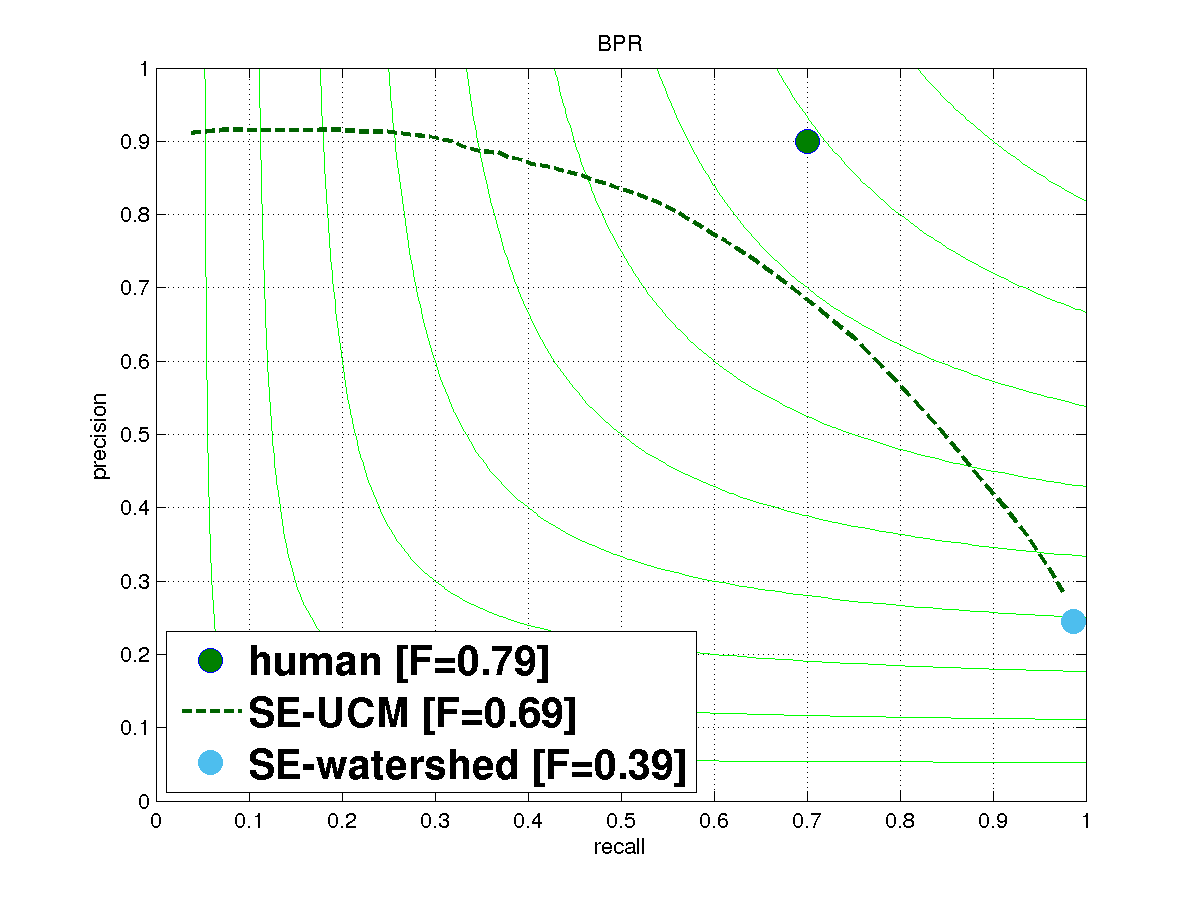
\includegraphics[trim=1.5cm 0cm 1.9cm 0cm, clip=true, width=0.48\textwidth]{images/plots/SE-watershed_BPR.png}
 }
 \subfigure[VPR]{%
  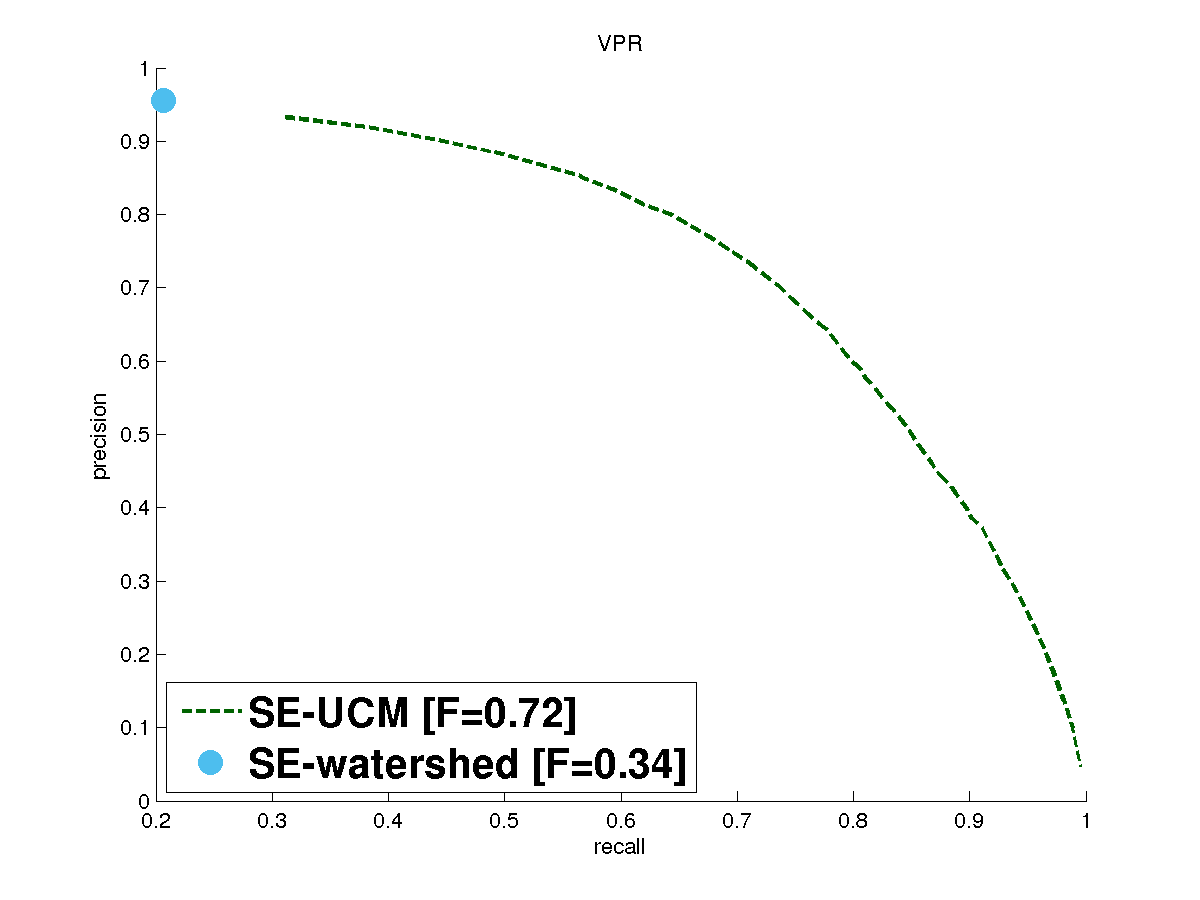
\includegraphics[trim=1.5cm 0cm 1.9cm 0cm, clip=true, width=0.48\textwidth]{images/plots/SE-watershed_VPR.png}
 }
\caption[SE-watershed and baseline: SE-UCM plots]{{\bf SE-watershed} provides a single oversegmentation. Our {\bf baseline - SE-UCM} is a UCM hierarchy built on top of the probability of boundary output of the SE edge detector.}
\label{fig:SE-watershed}
\end{figure}

\textbf{A point at issue % problem, trouble 
with non-maximum suppressed edges:} Note that the SE algorithm implements non-maximum suppression on the edge detection output to provide thinned edges. Non-maximum suppression is a method first introduced as a means of reducing thick edge responses to thin lines for the task of edge detection in greyscale images~\cite{rosenfeld1976digital}. Non-maximum suppression considers only the maxima in the gradient direction. As a consequence, the final output of the SE often has only single regional minimum. In the presence of a unique lake, the watershed is empty. To circumvent this problem, we use the SE detector \textit{before non-maxima suppression} as a topographic surface for the flooding.

\section{Baseline: SE-UCM}
As a baseline, we create a hierarchy of segmentations on top of the SE detector result. This is in the spirit of~\cite{Arbelaez2006boundary} who, however, use the edge detector of Martin, Fowlkes, and Malik (MFM)~\cite{martin2004learning}. What we do for this baseline could also be thought as our pipeline SE-SV-UCM without structured voting. Instead, the values from the probability of boundary, which is the output of the edge detector are directly transfered as values for the watershed pixels. Benchmark plots are on \fref{fig:SE-watershed}.

We observe the problem of strong edges ``bleeding'' into non-salient ones, despite lack of good local boundary evidence, as on the tikis examples (see \fref{fig:SE-UCM-tikis-bleeding-sub2}) between the heads of the middle and right statues. This issue is one of the motivations for the Structured voting (SV) described in \sref{sec:ch4-SE-SV-UCM_SV_details}.% Similarly

\begin{figure}[ht!]
\centering
\subfigure[Input image]{%
 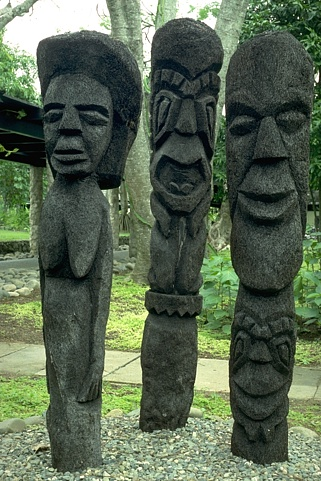
\includegraphics[width=0.3\textwidth]{images/examples/tikis/tikis.jpg}
 \label{fig:SE-UCM-tikis-bleeding-sub1}
}
\subfigure[UCM]{%
 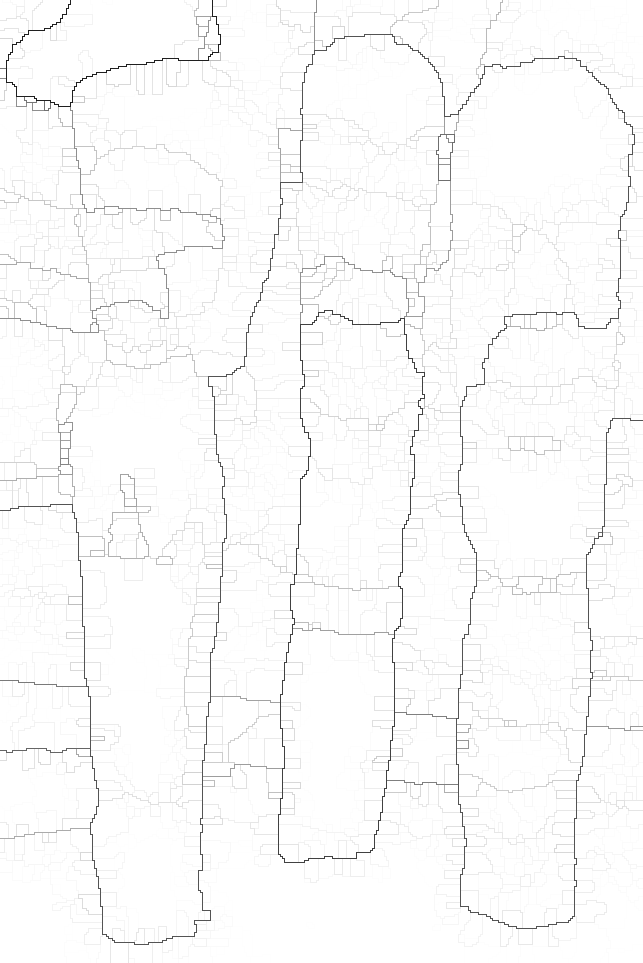
\includegraphics[width=0.3\textwidth,frame]{images/examples/tikis/SE-UCM-tikis-ucm-problem.png}
 \label{fig:SE-UCM-tikis-bleeding-sub2}
}
\caption[SE-UCM drawback - ``bleeding'' of strong edges towards unimportant ones]{{\bf SE-UCM} result. \protect\subref{fig:SE-UCM-tikis-bleeding-sub1} - an image from the validation subset of~\cite{BSDS500resources}. Notice how in the SE-UCM output \protect\subref{fig:SE-UCM-tikis-bleeding-sub2} unimportant horizontal edges between the statues' heads are {\it incorrectly %wrongly 
up-voted} due to strong vertical boundary in their vicinity (the outline of the statues).}
\label{fig:SE-UCM-tikis-bleeding}
\end{figure}
% BPR edge detector MFM 0.65, MFM-UCM 0.67 ; SE 0.70, % SE_no_nms_single_scale_repeat
% SE-UCM 0.69 (0.70)

\section{SE+sPb-UCM}
This experiment shows us that globalisation could easily be introduced to our method. Here we use the same affinity matrix as the spectral Pb of Arbel\'aez \etal~\cite{Arbelaez11}. Extending our algorithm to adopt a globalisation step could be beneficial, since it could pick up on improvements in the realm of spectral clustering, as for example spectral reduction~\cite{Galasso14}. % check the plots, check MCG paper - they did exactly this

\begin{figure}[ht!]
\centering
 \subfigure[BPR]{%
  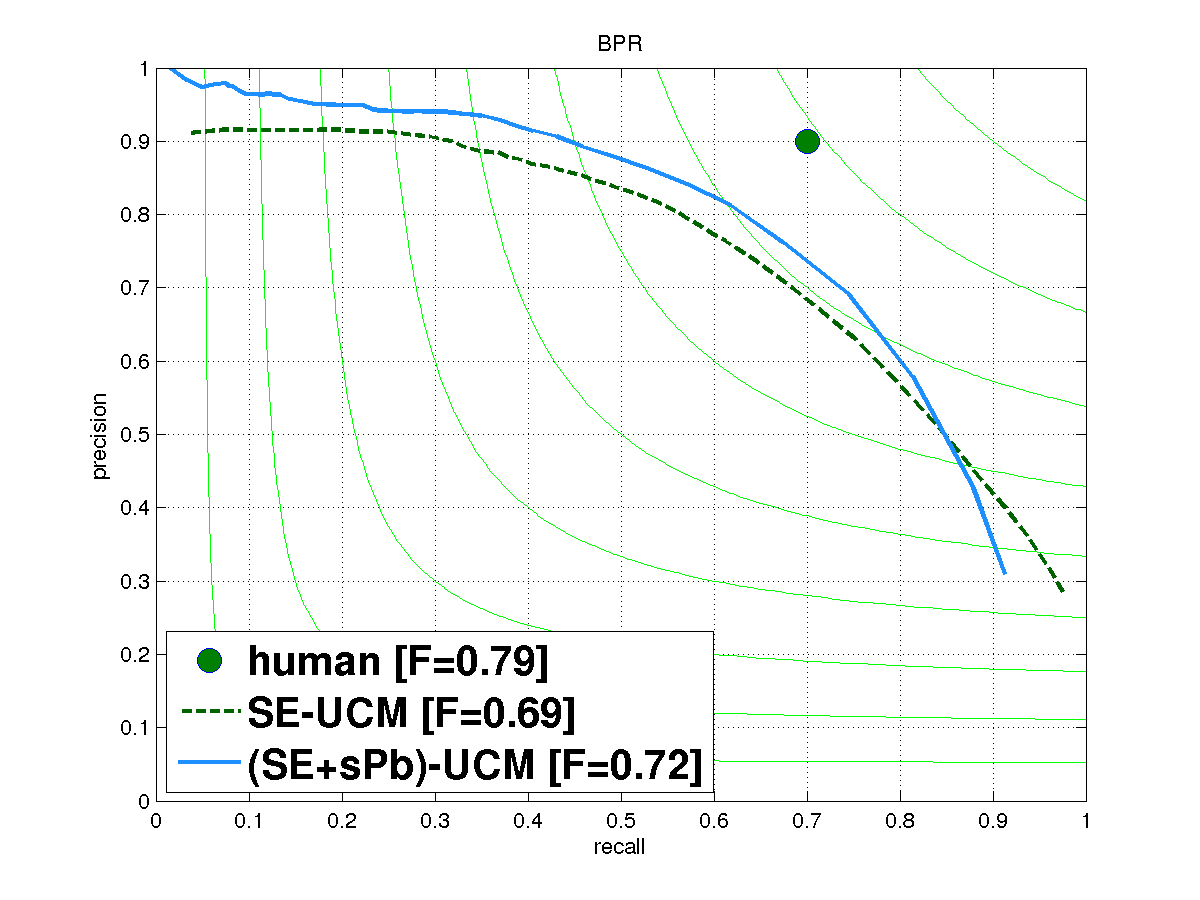
\includegraphics[trim=1.5cm 0cm 1.9cm 0cm, clip=true, width=0.48\textwidth]{images/plots/SE_nnms_sPb-UCM_BPR.png}
 }
 \subfigure[VPR]{%
  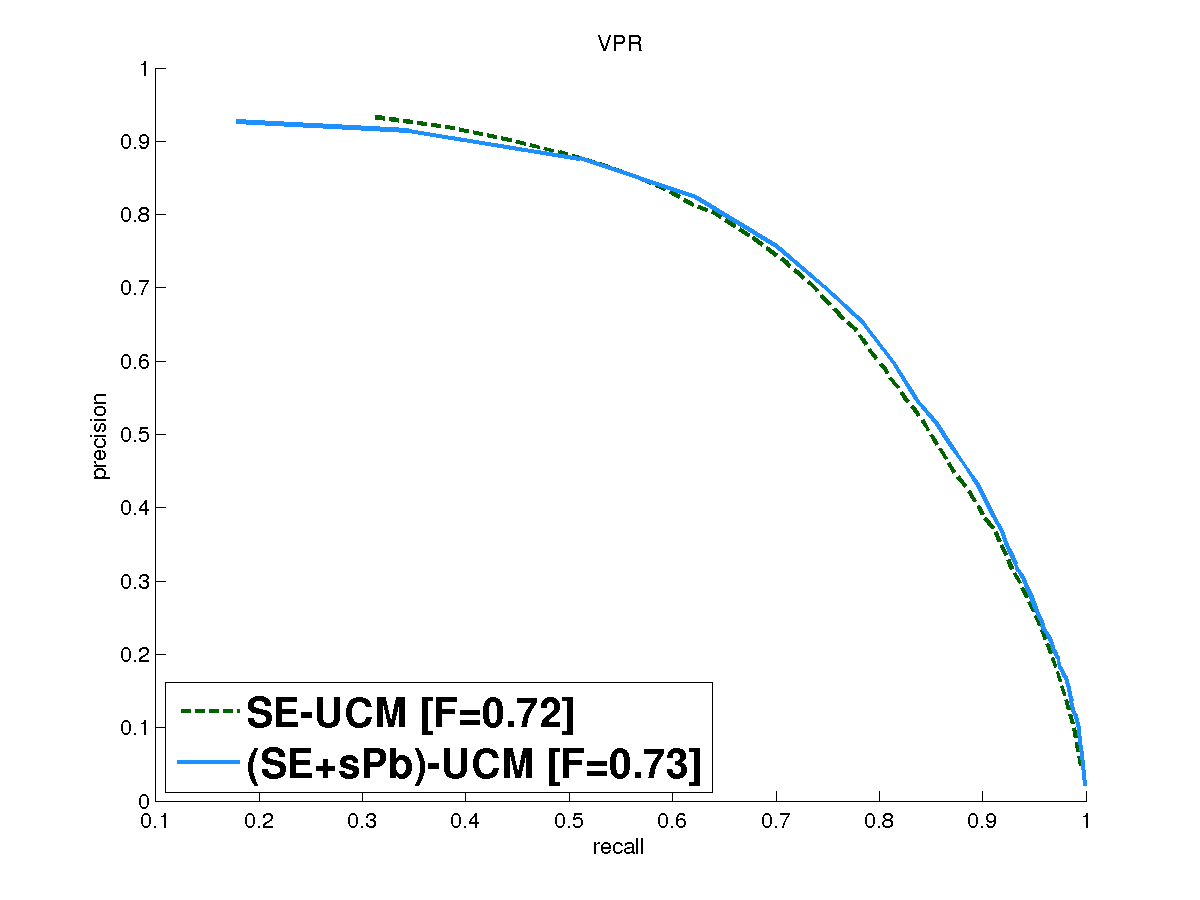
\includegraphics[trim=1.5cm 0cm 1.9cm 0cm, clip=true, width=0.48\textwidth]{images/plots/SE_nnms_sPb-UCM_VPR.png}
 }
\caption[(SE and spectralPb)-UCM plots]{SE+sPb-UCM.}
\label{fig:SE_nnms_sPb-UCM}
\end{figure}

% TODO here is a table of all results we will show. What to do with it, can't just dump all the data without proper analysis / conclusion?
\begin{table}[htbp]
\renewcommand{\arraystretch}{1.3}
\centering
\scriptsize
\begin{tabular}{l|c|c|c||c|c|c||c|c|c|}
\cline{2-10} % ZZ
\multirow{2}{*}{} & \multicolumn{3}{c||}{\textbf{BPR}} & \multicolumn{3}{c||}{\textbf{VPR}}& \multicolumn{3}{c|}{\textbf{Region}}\\
\cline{2-10}
& \textbf{ODS}  & \textbf{OIS} & \textbf{AP} % <- BPR
& \textbf{ODS} & \textbf{OSS} & \textbf{AP} % <- VPR
& \textbf{SC} & \textbf{PRI} & \textbf{VoI} \\
\hline
\multicolumn{1}{|c|}{Human} & .79 & .79 & - & - & - & - & .72 & .88 & 1.17 \\ % actually, we had .80 for humans on BPR from \cite{Arbelaez11}; % TODO for VPR - we don't know ODS = OIS for humans
\hline
\hline
\multicolumn{1}{|c|}{\cite{DollarICCV13edges} Structured edge (SE)} & .70 & .72 & .63 & - & - & - & - & - & - \\
\hline
\multicolumn{1}{|c|}{\cite{Arbelaez11} gPb-OWT-UCM} & .73 & .76 & .77 & .73 & .76 & .78 & .59 & .83 & 1.69 \\
\hline
\hline
\multicolumn{1}{|c|}{SE-watershed} & .39 & .39 & - & .34 & .34 & - & .20 & .75 & 6.26 \\
\hline
\multicolumn{1}{|c|}{SE-UCM (baseline)} & .69 &.73 & .75 & .72 & .75 & .77 & .58 & .82 & 1.80 \\
\hline
\multicolumn{1}{|c|}{SE+sPb-UCM} & .72 & .75 & .76 & .73 & .76 & .78 & .59 & .82 & 1.68 \\ % SE_nnms_sPb-UCM
\hline
\hline
\multicolumn{1}{|c|}{linear LLS} & .68 & .71 & .71 & .69 & .71 & .71 & .55 & .81 & 1.90 \\% linear model - linear least squares fitting}
\hline
\multicolumn{1}{|c|}{quadratic LLS} & .54 & .56 & .40 & .40 & .40 & .25 & .37 & .55 & 2.45 \\
\hline
\hline
\end{tabular}
\caption[All results]{Results of all our experiments.}
%The table shows aggregate measures (ODS, OSS, AP) for boundary precision-recall (BPR), volume precision-recall (VPR) and 
%includes region statistics (SC, PRI, VoI).}
\label{tab:all-results}
\end{table}

% quadratic
% Boundary PR global
%    G-ODS: F( R 0.57, P 0.52 ) = 0.54   [th = 0.12]
%    G-OIS: F( R 0.57, P 0.54 ) = 0.56
%    Area_PR = 0.40
% Volume PR global
%    G-ODS: F( R 0.79, P 0.27 ) = 0.40   [th = 0.02]            <- NOTE: very low threshold! can't recall all boundaries, that explains the plot
%    G-OSS: F( R 0.79, P 0.26 ) = 0.40
%    G-Area_PR = 0.25
% Region
%    GT covering: ODS = 0.34 [th = 0.21]. OSS = 0.35. Best = 0.37
% Region
%    Rand Index: ODS = 0.55 [th = 0.02]. OSS = 0.55.
%    Var. Info.: ODS = 2.45 [th = 0.73]. OSS = 2.37.


% SE-UCM baseline
% Boundary PR global
%    G-ODS: F( R 0.70, P 0.69 ) = 0.69   [th = 0.27]
%    G-OIS: F( R 0.73, P 0.73 ) = 0.73
%    Area_PR = 0.75
% Volume PR global
%    G-ODS: F( R 0.71, P 0.73 ) = 0.72   [th = 0.25]
%    G-OSS: F( R 0.73, P 0.77 ) = 0.75
%    G-Area_PR = 0.77
% Region
%    GT covering: ODS = 0.58 [th = 0.29]. OSS = 0.64. Best = 0.73
% Region
%    Rand Index: ODS = 0.82 [th = 0.17]. OSS = 0.86.
%    Var. Info.: ODS = 1.80 [th = 0.52]. OSS = 1.57.

% SE_nnms_sPb-UCM
% Boundary PR global
%    G-ODS: F( R 0.72, P 0.72 ) = 0.72   [th = 0.08]
%    G-OIS: F( R 0.74, P 0.76 ) = 0.75
%    Area_PR = 0.76
% Volume PR global
%    G-ODS: F( R 0.70, P 0.76 ) = 0.73   [th = 0.10]
%    G-OSS: F( R 0.74, P 0.77 ) = 0.76
%    G-Area_PR = 0.78
% Region
%    GT covering: ODS = 0.59 [th = 0.12]. OSS = 0.64. Best = 0.74
% Region
%    Rand Index: ODS = 0.82 [th = 0.08]. OSS = 0.85.
%    Var. Info.: ODS = 1.68 [th = 0.15]. OSS = 1.48.

% linear LLS
% Boundary PR global
%    G-ODS: F( R 0.69, P 0.67 ) = 0.68   [th = 0.35]
%    G-OIS: F( R 0.74, P 0.67 ) = 0.71
%    Area_PR = 0.71
% Volume PR global
%    G-ODS: F( R 0.68, P 0.70 ) = 0.69   [th = 0.27]
%    G-OSS: F( R 0.70, P 0.73 ) = 0.71
%    G-Area_PR = 0.71
% Region
%    GT covering: ODS = 0.55 [th = 0.37]. OSS = 0.60. Best = 0.67
% Region
%    Rand Index: ODS = 0.81 [th = 0.17]. OSS = 0.83.
%    Var. Info.: ODS = 1.90 [th = 0.67]. OSS = 1.72.

% quadratic LLS
% Boundary PR global
%    G-ODS: F( R 0.57, P 0.52 ) = 0.54   [th = 0.12]
%    G-OIS: F( R 0.57, P 0.54 ) = 0.56
%    Area_PR = 0.40
% Volume PR global
%    G-ODS: F( R 0.79, P 0.27 ) = 0.40   [th = 0.02]
%    G-OSS: F( R 0.79, P 0.26 ) = 0.40
%    G-Area_PR = 0.25
% Region
%    GT covering: ODS = 0.34 [th = 0.21]. OSS = 0.35. Best = 0.37


\section[Structured voting]{Structured voting - experimental study of watershed weighting strategies}
\label{sec:ch5-structured-voting}
All experiments presented here are instances of the general algorithm described in \sref{sec:ch4-SE-SV-UCM_SV_details}.

% \settocdepth{section}
% \settocdepth{subsection}
\settocdepth{section}
\subsection{Superpixels and Rand index}
We leave the watershed patch to be an oversegmentation, which in fact it is. The output of the watershed transform that we use has explicit the boundaries between segments, which would hinder a region-based metric. Therefore, we transform a watershed patch to have implicit segment boundaries - the locations of transition between differently labelled segments. 
The patches from the decision forest already constitute segmentation labelling with implicit segment boundaries. That, of course, is due to the fact that the structured forest patches are taken unmodified from the ground truth segmentations of the training subset of BSDS500, which has a ``labelling with implicit segment boundaries'' format. We conduct the comparison between watershed and a tree leaf patch using as a scoring function:

\begin{itemize}
 \item{\bf Rand Index (RI):} a count of the number of pairs of locations that belong to the same segment in both patches. For a $16\times16$ segmentation patch, that means $32 640$ pairs of locations.
 \item{\bf Rand Index Monte Carlo (RIMC):} ours randomised subsample version of RI, which takes only a fraction $\rho$ of the pairs of locations into consideration. We experience no reduction in performance \wrt RI for a fraction as small as $\rho\approx\frac{1}{128}$, \ie, 256 out of the $32 640$ possible pairs of locations in a $16 \times 16$ patch. This scoring function is inspired from the way features are subsampled to introduce randomness when training a decision tree in~\cite{DollarICCV13edges,Dollar2013toolbox}.
\end{itemize}

The above experiments (both having a result of $F=0.55$ on BPR) led us to two conclusions. First, we need to have a closer look into the properties of our \textbf{scoring functions}. Section~\ref{sec:ch4-boundary-and-region-metrics-maths} of the previous chapter gives mathematical formulae and a detailed explanation on the metrics we considered for this task. Second, a \textbf{simplification of the watershed patch} is desirable, due to the discrepancy %mismatch between 
in makeup %constitution
of watershed and decision tree patches.

\subsection{Na\"{\i}ve greedy merge of watershed patch}
We first address the second of our conclusions from the previous experiment. We merge segments in the watershed patch according to each of the $T$ leaf patches (where $T$ is the number of trees in the decision forest). Thus we end up with $T$ distinct ``merged'' watershed patches. This approach seems to be too greedy, however. The watershed patch eventually becomes overly adapted to the tree leaf patch it is being compared to. As a consequence, this watershed transformation is not discriminative enough.

\subsubsection{Fair greedy merge}
To remedy this shortcoming of the na\"{\i}ve greedy merge, we introduce what we call ``fairness'' in the greedy merge approach. As described previously, we cast votes only on the watershed locations. That means, the patches that we consider contain a potential boundary location at their central pixel. It is the strength of this boundary that we strive to quantify. We enforce the greedy merge to respect a boundary-at-centre-location condition by preventing excessive merge of the segments around the central pixel of the patch.
% TODO image of the patches

\fref{fig:segs-to-greedy-merge-RIMC} shows the improvement we get over watershed oversegmentation with the last two experiments.

\begin{figure}[ht!]
\centering
 \subfigure[BPR]{%
  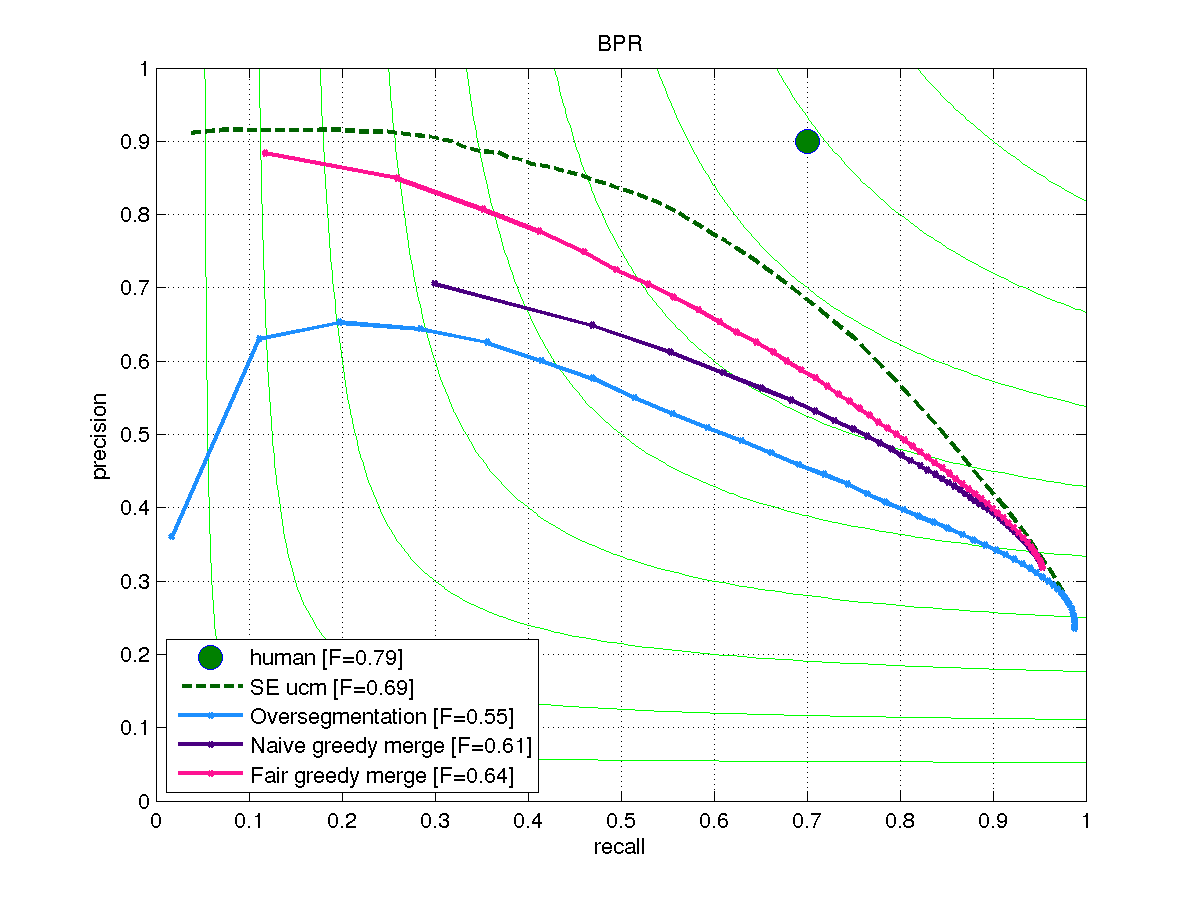
\includegraphics[trim=1.5cm 0cm 1.9cm 0cm, clip=true, width=0.48\textwidth]{images/plots/segs-to-greedy-merge-RIMC-BPR.png}
 }
 \subfigure[VPR]{%
  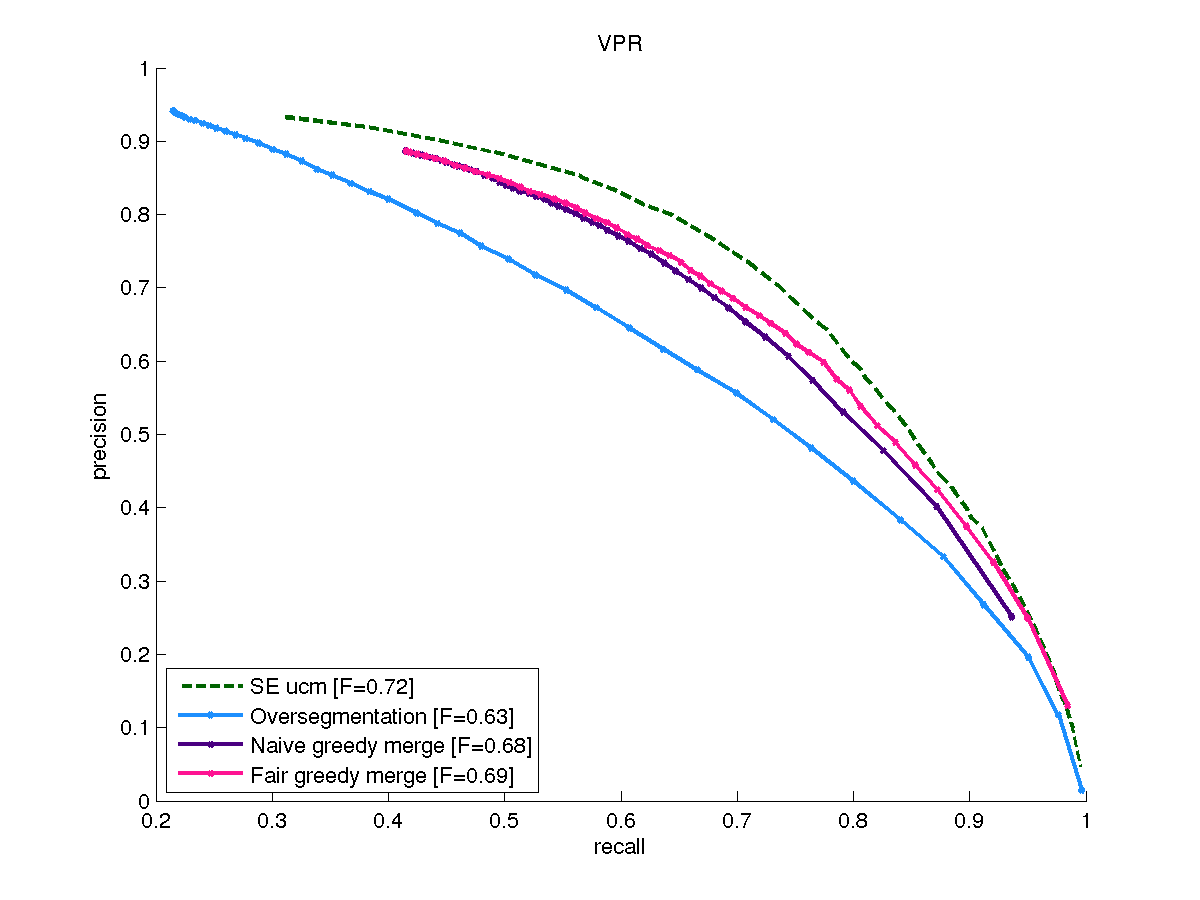
\includegraphics[trim=1.5cm 0cm 1.9cm 0cm, clip=true, width=0.48\textwidth]{images/plots/segs-to-greedy-merge-RIMC-VPR.png}
 }
\caption[Greedy merge experiments]{Greedy merge experiments. In all cases the scoring function used for patches comparison was the RIMC (Section~\ref*{sec:ch4-boundary-and-region-metrics-maths}~\ref{par:ch4-RIMC-maths} contains a description of the RIMC metric).} % (\hyperref[par:ch4-RIMC-maths]{RIMC description in Chapter 4}).} % that looks bad on paper, still useful for .pdf, as it contains the link
\label{fig:segs-to-greedy-merge-RIMC}
\end{figure}

\subsection{Watershed region boundary}
We would like our watershed weighting strategy to take into account fine changes in the shape of the region boundary. To this end, we transform the watershed patch to contain exclusively the part of the watershed on which we are to cast our vote, and discard all other region boundaries present in the patch.

This approach does not guarantee closed contours - the part of the region boundary present in the patch would often be \textbf{just an image edge}. So we cannot use as a scoring function a region metric but must instead use a boundary-based one. We must, therefore, transform the segmentation patch from the tree leaf to a boundary patch. It is trivial~\cite{Arbelaez11} to obtain an edge map, given a segmentation. our transformed tree leaf patch is a binary edge map. As a scoring function we use the our boundary-based evaluation metric - BPR.

% BPR on contours - watershed arc and region boundary
Our conclusion from this experiment is that the combination of only the edge with the BPR provides poor means of judging the evidence of boundary in the leaves of the structured forest. Watershed region boundary is a very brittle cue. Further, BPR is parametrised on the pixel distance for which a match between the two segmentation boundaries is to be made. There is not a generic way to correctly choose such a distance for all forest segmentation patches and watershed locations. Accurate localisation of boundaries seems to be crucial for this weighting strategy, and this is not the case with the leaf segmentations and the watershed.

\subsection{Line fitting}
Our best performing weighting strategy. We implemented three line fitting algorithms:
\begin{enumerate}
  \item parametric, based on the derivative direction of the end-points of the watershed edge we vote on,
  \item as above, but enforcing adherence to the centre of the image patch,
  \item linear least squares fitting to all the watershed edge pixels.
 % also possible - PCA-based fit
\end{enumerate}

Discuss performance \wrt different scoring functions. Notable that all 3 types of scoring functions - VPR, RI, BPR perform reasonably well with this watershed transformation. Normalisation of VPR. Asymmetry of normalisation and how it affects us.

\subsection{Quadratic fitting} % conic n=2; Polynomial
Conic sections - parabola, hyperbola and ellipse that fit the data. Too complex a model, thwarted by degenerate cases (best fitting parameters yield a 3-dimensional surface that doesn't intersect the $Z=0$ plane).


\begin{figure}[ht!]
\centering
 \subfigure[BPR]{%
  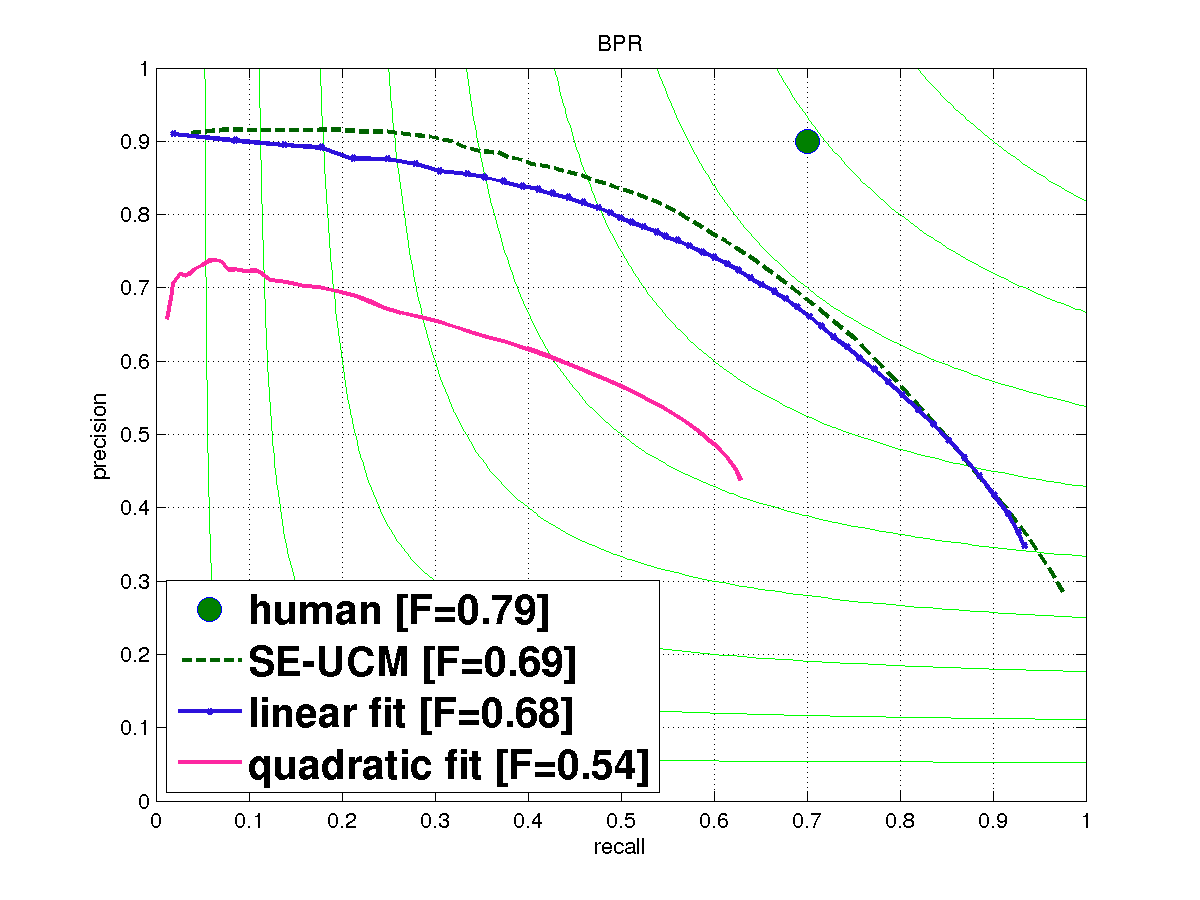
\includegraphics[trim=1.5cm 0cm 1.9cm 0cm, clip=true, width=0.48\textwidth]{images/plots/SE-quadratic_BPR.png}
 }
 \subfigure[VPR]{%
  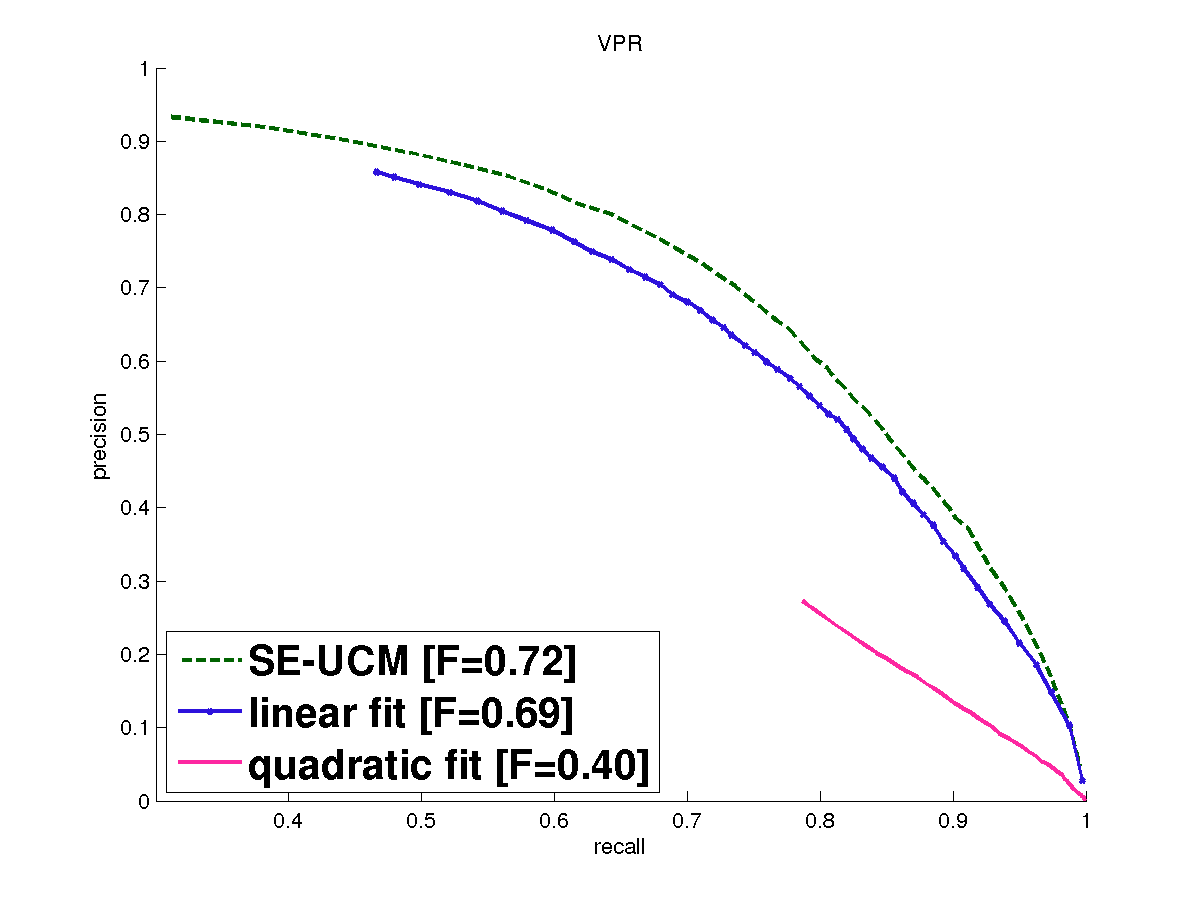
\includegraphics[trim=1.5cm 0cm 1.9cm 0cm, clip=true, width=0.48\textwidth]{images/plots/SE-quadratic_VPR.png}
 }
\caption[Quadratic linear least squares fitting compared to the linear model - plots]{{\bf Quadratic} linear least squares fitting compared to the {\bf linear} model. The scoring function for the two experiments was the VPR normalised on the side of the watershed.}
\label{fig:SE-quadratic}
\end{figure}

\settocdepth{subsection}
\section[Oracle for Structured voting]{Oracle for SV - experiments using ground truth}
\label{sec:ch5-oracle}
To evaluate the correctness of our weighting strategies, we've implemented an oracle for our pipeline. The question we wanted to answer is ``how well could we perform segmentation in the presence of perfect information?'' Our Structured voting lends itself easily to such an experiment using the ground truth segmentation. 
When scoring a given pixel on the watershed regions boundary, we use a ground truth segmentation patch, rather than the most likely segmentation learnt by the structured forest. The second patch, as in the regular experiments, is taken from the same pixel location in the watershed locations image.

\section{Hardest negative mining}
Help determine where the voting fails the most. Conclusion: with so few votes per location, our approach would need much better leaves. We observed a lack of strong agreement in the leaves of the decision forest. The medoid segmentation patch, which is the only one casting a vote, is not necessarily representative of the set of segmentations that reached the leaf node of the tree.
% TODO figure of decision forest leaf, pref. different leaves

\section{Voting scope}
% TODO two types of voting scope experiments - reducing and expanding; two plots
  \begin{itemize}
    \item{\bf Degraded baseline SE-UCM:} Have the SF output a pixel, or a $2\times2$, $4\times4$, $8\times8$ patch.
    \item{\bf Reduced vote scope:} This series of experiments aims at proving that casting a vote on a larger area is desireable, by doing exactly the opposite. We cast just $T$ votes ($T$ - number of trees in the decision forest) on a single pixel of the watershed location. As expected, that severely diminishes performance (\wrt averaging on the region boundary) since the voting scope is decreased to 1 pixel. Excessive localisation therefore hinders performance.
  \end{itemize}
Discussion: It would be useful to see the effect of a ``mixed'' scope of voting - cast vote on the whole region boundary, but use subdivided region boundary - the watershed arc in order to do the patch transformation.

\begin{figure}[ht!]
\centering
 \subfigure[BPR]{%
  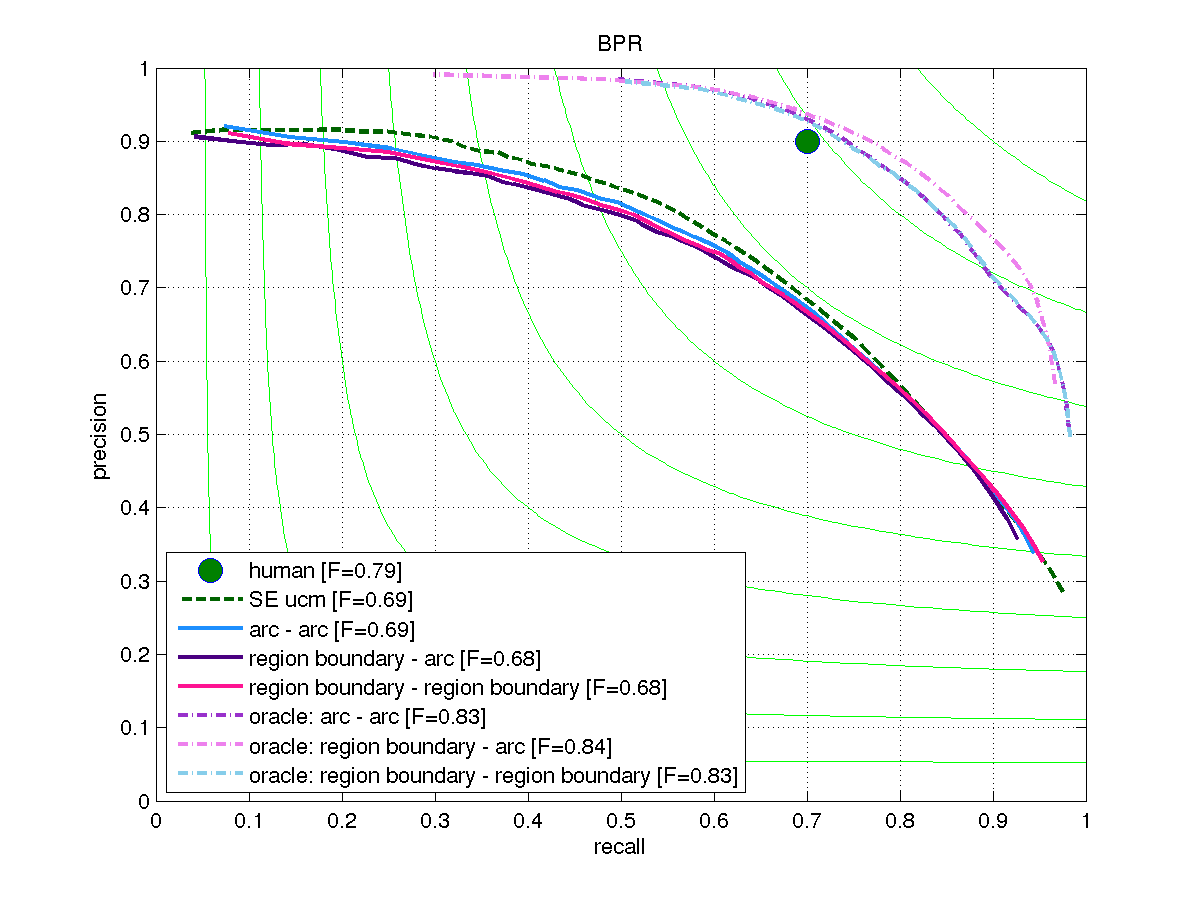
\includegraphics[trim=1.5cm 0cm 1.9cm 0cm, clip=true, width=0.48\textwidth]{images/plots/scope_of_voting_oracle_disagreement__line_centre_VPR_ws_BPR.png}
 }
 \subfigure[VPR]{%
  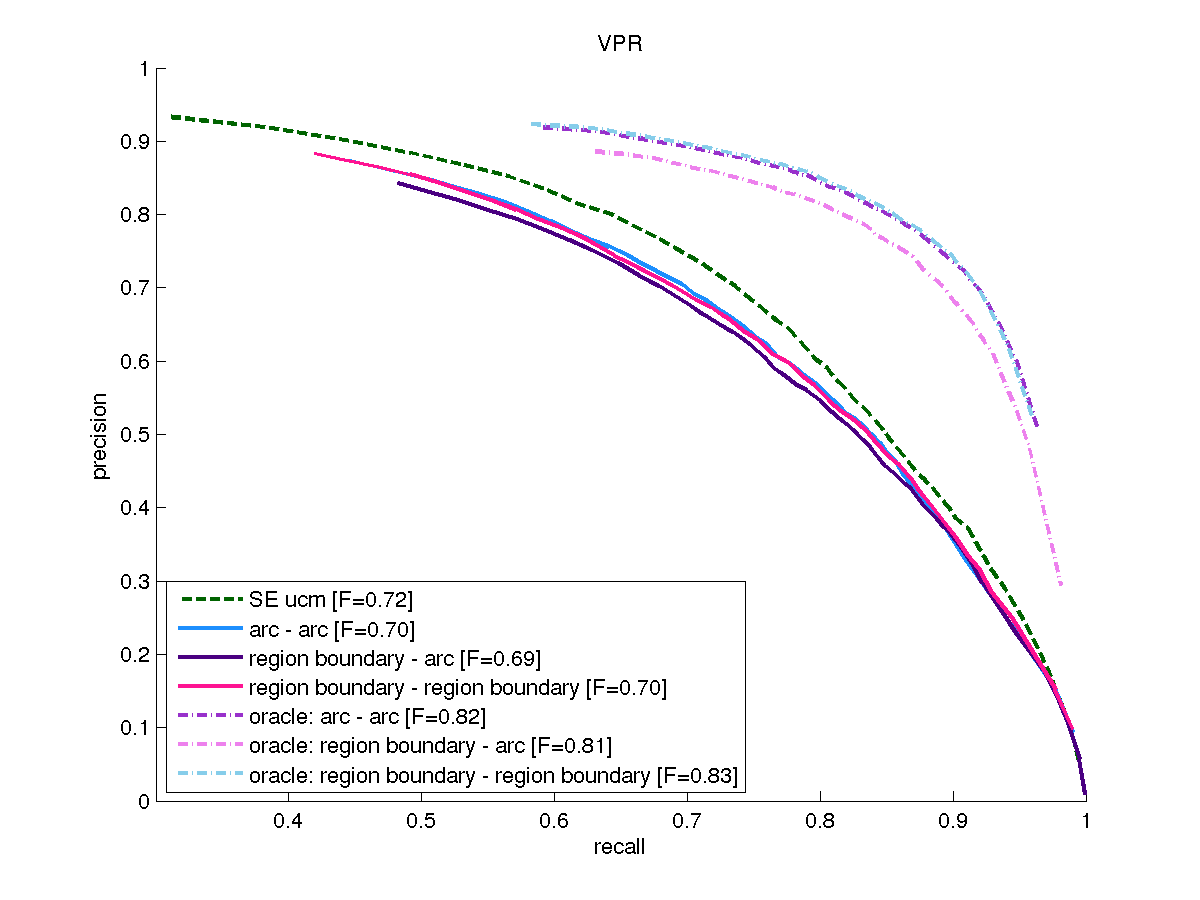
\includegraphics[trim=1.5cm 0cm 1.9cm 0cm, clip=true, width=0.48\textwidth]{images/plots/scope_of_voting_oracle_disagreement__line_centre_VPR_ws_VPR.png}
 }
\caption[Voting scope experiments.]{Voting scope experiments. The three segmentation methods and their oracles are variants of our best performing weighting strategy - central line fitting, cobined with VPR normalised on the side of the watershed. A description of VPR is given in Section~\ref*{sec:ch4-boundary-and-region-metrics-maths}~\ref{par:ch4-VPR-maths}).}
\label{fig:voting-scope-line-centre-VPR-ws}
\end{figure}

\section{Discussion}

Important conclusions of the experiments:
\begin{enumerate}
 \item both watershed transformations and scoring functions are important,
 % \item scoring functions matter,
 \item a suitable %smart
 watershed transformation could greatly aid a ``weaker'' scoring function (\eg the benefit of greedy merge when using RI scoring function),
 \item our best watershed transformation has reasonable performance with all the scoring functions tried,
 \item oracle confirms the ranking of our experiments,
 \item simpler models work better for transforming the watershed patch (\eg quadratic and polynomial fitting are the worst performing experiments regardless of the scoring function used),
 \item voting scope is very important; a decrease in the voting scope seriously damages results; successfully increasing the voting scope is not trivial.
\end{enumerate}